\documentclass[border=2pt]{standalone}
\usepackage{pgfplots}
\usepgfplotslibrary{colorbrewer}
\usetikzlibrary{shapes,arrows}

\begin{document}

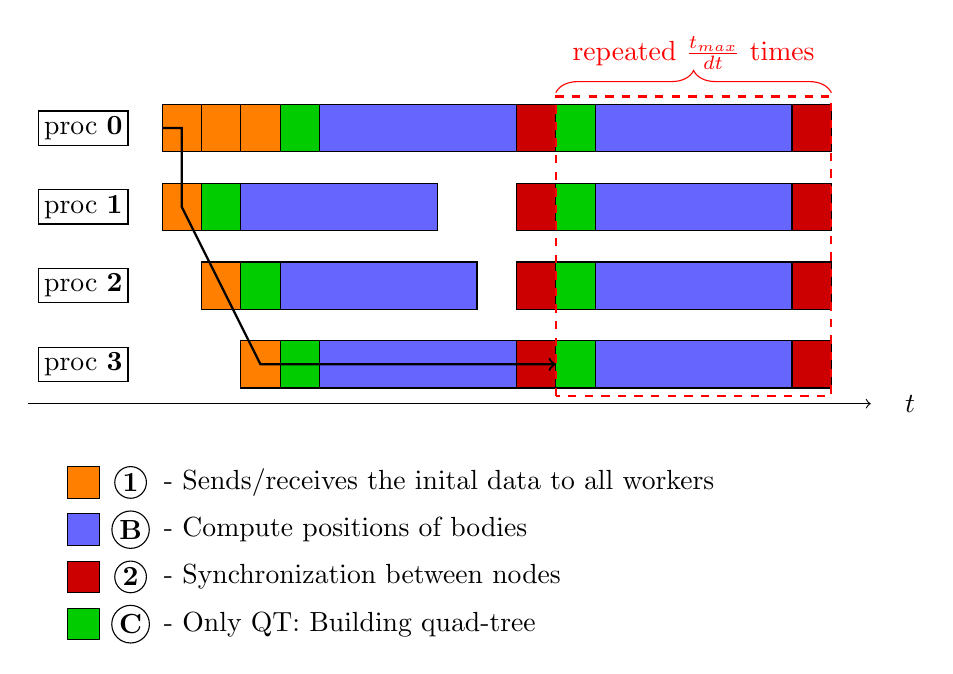
\begin{tikzpicture}
  \def\bottomAlign{-0.3};
  \def\height{0.6};
  \def\vspace{-1.0};

  \def\leftAlign{1.0};
  \def\loadingTime{0.0};
  \def\sendingTime{0.5};
  \def\computeTime{2.5};
  \def\buildingTime{0.5};

  \def\endInitial{5.5};

  \node (startLoading) at (\leftAlign,0){};
  \node (middleReceiv0) at (\leftAlign + \loadingTime + 0.5*\sendingTime,0){};
  \node (middleReceiv1) at (\leftAlign + \loadingTime + 0.5*\sendingTime,1*\vspace){};
  \node (middleReceiv2) at (\leftAlign + \loadingTime + 1.5*\sendingTime,2*\vspace){};
  \node (middleReceiv3) at (\leftAlign + \loadingTime + 2.5*\sendingTime,3*\vspace){};
  \node (middleReceivFinal3) at (\endInitial + \sendingTime,3*\vspace){};
%  \node (middleReceivFinal3) at (\endInitial + \sendingTime + \buildingTime + \computeTime + \sendingTime,3*\vspace){};
  \node (middleReceivFinal0) at (\endInitial + \sendingTime + \buildingTime + \computeTime + \sendingTime,0){};


  \node[draw,rectangle,inner sep=2pt] at (0,0.0) {proc \textbf{0}};
  \node[draw,rectangle,inner sep=2pt] at (0,-1) {proc \textbf{1}};
  \node[draw,rectangle,inner sep=2pt] at (0,-2) {proc \textbf{2}};
  \node[draw,rectangle,inner sep=2pt] at (0,-3) {proc \textbf{3}};
  
  % proc 0
  \filldraw[yellow!90!black, draw = black] (\leftAlign,\bottomAlign) rectangle (\leftAlign + \loadingTime, \bottomAlign + \height);

  \filldraw[orange, draw=black] (\leftAlign + \loadingTime,\bottomAlign) rectangle (\leftAlign + \loadingTime + \sendingTime,\bottomAlign + \height);
  \filldraw[orange, draw=black] (\leftAlign + \loadingTime + \sendingTime,\bottomAlign) rectangle (\leftAlign + \loadingTime + 2*\sendingTime,\bottomAlign + \height);
  \filldraw[orange, draw=black] (\leftAlign + \loadingTime + 2*\sendingTime,\bottomAlign) rectangle (\leftAlign + \loadingTime + 3*\sendingTime,\bottomAlign + \height);
  \filldraw[green!80!black, draw=black] (\leftAlign + \loadingTime + 3*\sendingTime,\bottomAlign) rectangle (\leftAlign + \loadingTime + 3*\sendingTime + \buildingTime, \bottomAlign + \height);


  \filldraw[blue!60!white, draw=black] (\leftAlign + \loadingTime + 3*\sendingTime + \buildingTime, \bottomAlign) rectangle (\leftAlign + \loadingTime + 3*\sendingTime + \buildingTime + \computeTime,\bottomAlign + \height);
  \filldraw[red!80!black, draw=black] (\endInitial,\bottomAlign) rectangle (\endInitial + \sendingTime,\bottomAlign + \height);
  \filldraw[green!80!black, draw=black] (\endInitial + \sendingTime,\bottomAlign) rectangle (\endInitial + \sendingTime + \buildingTime,\bottomAlign + \height);

  \filldraw[blue!60!white, draw=black] (\endInitial + \sendingTime + \buildingTime,\bottomAlign) rectangle (\endInitial + \sendingTime + \buildingTime + \computeTime,\bottomAlign + \height);
  \filldraw[red!80!black, draw=black] (\endInitial + \sendingTime + \buildingTime + \computeTime,\bottomAlign) rectangle (\endInitial + \sendingTime + \buildingTime + \computeTime + \sendingTime,\bottomAlign + \height);

  % proc 1
  \filldraw[orange, draw=black] (\leftAlign + \loadingTime , \vspace + \bottomAlign) rectangle (\leftAlign + \loadingTime + \sendingTime, \vspace + \bottomAlign + \height);
  \filldraw[green!80!black, draw=black] (\leftAlign + \loadingTime + 1*\sendingTime, 1*\vspace + \bottomAlign) rectangle (\leftAlign + \loadingTime + 1*\sendingTime + \buildingTime,  1*\vspace + \bottomAlign + \height);
  \filldraw[blue!60!white, draw=black] (\leftAlign + \loadingTime + \sendingTime + \buildingTime, \vspace + \bottomAlign) rectangle (\leftAlign + \loadingTime + \sendingTime + \buildingTime + \computeTime, \vspace + \bottomAlign + \height);

  \filldraw[red!80!black, draw=black] (\endInitial,\vspace + \bottomAlign) rectangle (\endInitial + \sendingTime, \vspace + \bottomAlign + \height);
  \filldraw[green!80!black, draw=black] (\endInitial + \sendingTime, \vspace + \bottomAlign) rectangle (\endInitial + \sendingTime + \buildingTime, \vspace + \bottomAlign + \height);
  \filldraw[blue!60!white, draw=black] (\endInitial + \sendingTime + \buildingTime, \vspace + \bottomAlign) rectangle (\endInitial + \sendingTime + \buildingTime + \computeTime, \vspace + \bottomAlign + \height);
  \filldraw[red!80!black, draw=black] (\endInitial + \sendingTime + \buildingTime + \computeTime, \vspace + \bottomAlign) rectangle (\endInitial + \sendingTime + \buildingTime + \computeTime + \sendingTime, \vspace + \bottomAlign + \height);
  % proc 2
  \filldraw[orange, draw=black] (\leftAlign + \loadingTime + \sendingTime, 2*\vspace + \bottomAlign) rectangle (\leftAlign + \loadingTime + 2*\sendingTime, 2*\vspace + \bottomAlign + \height );
  \filldraw[green!80!black, draw=black] (\leftAlign + \loadingTime + 2*\sendingTime, 2*\vspace + \bottomAlign) rectangle (\leftAlign + \loadingTime + 2*\sendingTime + \buildingTime,  2*\vspace + \bottomAlign + \height);

  \filldraw[blue!60!white, draw=black] (\leftAlign + \loadingTime + 2*\sendingTime + \buildingTime, 2*\vspace + \bottomAlign) rectangle (\leftAlign + \loadingTime + 2*\sendingTime + \buildingTime + \computeTime, 2*\vspace + \bottomAlign + \height);

  \filldraw[red!80!black, draw=black] (\endInitial,2*\vspace + \bottomAlign) rectangle (\endInitial + \sendingTime, 2*\vspace + \bottomAlign + \height);
  \filldraw[green!80!black, draw=black] (\endInitial + \sendingTime, 2*\vspace + \bottomAlign) rectangle (\endInitial + \sendingTime + \buildingTime, 2*\vspace + \bottomAlign + \height);
  \filldraw[blue!60!white, draw=black] (\endInitial + \sendingTime + \buildingTime, 2*\vspace + \bottomAlign) rectangle (\endInitial + \sendingTime + \buildingTime + \computeTime, 2*\vspace + \bottomAlign + \height);
  \filldraw[red!80!black, draw=black] (\endInitial + \sendingTime + \buildingTime + \computeTime, 2*\vspace + \bottomAlign) rectangle (\endInitial + \sendingTime + \buildingTime + \computeTime + \sendingTime, 2*\vspace + \bottomAlign + \height);

  % proc 3
  \filldraw[orange, draw=black] (\leftAlign + \loadingTime + 2*\sendingTime, 3*\vspace + \bottomAlign) rectangle (\leftAlign + \loadingTime + 3*\sendingTime, 3*\vspace + \bottomAlign + \height );
  \filldraw[green!80!black, draw=black] (\leftAlign + \loadingTime + 3*\sendingTime, 3*\vspace + \bottomAlign) rectangle (\leftAlign + \loadingTime + 3*\sendingTime + \buildingTime,  3*\vspace + \bottomAlign + \height);

  \filldraw[blue!60!white, draw=black] (\leftAlign + \loadingTime + 3*\sendingTime + \buildingTime, 3*\vspace + \bottomAlign) rectangle (\leftAlign + \loadingTime + 3*\sendingTime  + \buildingTime+ \computeTime, 3*\vspace + \bottomAlign + \height);

  \filldraw[red!80!black, draw=black] (\endInitial, 3*\vspace + \bottomAlign) rectangle (\endInitial + \sendingTime, 3*\vspace + \bottomAlign + \height);
  \filldraw[green!80!black, draw=black] (\endInitial + \sendingTime, 3*\vspace + \bottomAlign) rectangle (\endInitial + \sendingTime + \buildingTime, 3*\vspace + \bottomAlign + \height);
  \filldraw[blue!60!white, draw=black] (\endInitial + \sendingTime + \buildingTime, 3*\vspace + \bottomAlign) rectangle (\endInitial + \sendingTime + \buildingTime + \computeTime, 3*\vspace + \bottomAlign + \height);
  \filldraw[red!80!black, draw=black] (\endInitial + \sendingTime + \buildingTime + \computeTime, 3*\vspace + \bottomAlign) rectangle (\endInitial + \sendingTime + \buildingTime + \computeTime + \sendingTime, 3*\vspace + \bottomAlign + \height);

  \draw[red, dashed, thick] (\endInitial + \sendingTime,-3.4) rectangle (\endInitial + \sendingTime + \buildingTime + \computeTime + \sendingTime, 0.4);
  \draw [red,decorate,decoration={brace,amplitude=8pt}] (\endInitial + \sendingTime, 0.45) -- node [pos=0.5, midway, yshift=0.5cm] {repeated $\frac{t_{max}}{dt}$ times} (\endInitial + \sendingTime + \buildingTime + \computeTime + \sendingTime,0.45);

  \draw[->] (-0.7, -3.5) -- (\endInitial + \sendingTime + \buildingTime + \computeTime + \sendingTime + 0.5 ,-3.5) node[xshift=0.5cm] {$t$};

  % critical path
  \draw [->,thick] (startLoading.center) -- (middleReceiv0.center) -- (middleReceiv1.center) -- (middleReceiv2.center) -- (middleReceiv3.center) -- (middleReceivFinal3.center);

  % legend
  %\filldraw[yellow!90!black, draw = black] (-0.2,-4.1) rectangle (0.2,-3.7);
  \filldraw[orange, draw=black] (-0.2,-4.7) rectangle (0.2,-4.3);
  \filldraw[blue!60!white, draw=black] (-0.2,-5.3) rectangle (0.2,-4.9);
  \filldraw[red!80!black, draw=black] (-0.2,-5.9) rectangle (0.2,-5.5);
  \filldraw[green!80!black, draw=black] (-0.2,-6.5) rectangle (0.2,-6.1);
  
  %\node[draw,circle,inner sep=1pt] at (0.6,-3.9) {\textbf{A}};
  \node[draw,circle,inner sep=1pt] at (0.6,-4.5) {\textbf{1}};
  \node[draw,circle,inner sep=1pt] at (0.6,-5.1) {\textbf{B}};
  \node[draw,circle,inner sep=1pt] at (0.6,-5.7) {\textbf{2}};
  \node[draw,circle,inner sep=1pt] at (0.6,-6.3) {\textbf{C}};

  %\node[right] at (0.9,-3.9) {- Loads inital data};
  \node[right] at (0.9,-4.5) {- Sends/receives the inital data to all workers};
  \node[right] at (0.9,-5.1) {- Compute positions of bodies};
  \node[right] at (0.9,-5.7) {- Synchronization between nodes};
  \node[right] at (0.9,-6.3) {- Only QT: Building quad-tree};

\end{tikzpicture}
\end{document}
